\documentclass[xcolor=pdftex,dvipsnames]{beamer}

\usepackage{amsmath}
\usepackage{amssymb}
\usepackage{comment}
\usepackage{textcomp}

\DeclareRobustCommand{\rsout}[1]{\texorpdfstring{\sout{#1}}}

\title{Microeconomic Theory --- ECON 323 503 \\ Chapter 17: Property
  Rights, Externalities, Rivalry, and Exclusion}
\author{Vikram Manjunath}       %
\institute{Texas A\&M University}
\setbeamertemplate{navigation symbols}{}
\setbeamertemplate{footline}{}
\usefonttheme{serif}
\begin{document}

\maketitle

\begin{frame}
\frametitle{Outline}
\begin{enumerate}[<+->]
\item Externalities: One may not take account of how his actions
  affect others.
\item The inefficiency of competition with externalities: Private
  incentives don't lead to the right amount of a good that causes externalities.
\item Regulating externalities: The inefficiency can be corrected by regulation.
\item Market structure and externalities: How does the picture change
  if the market isn't competitive?
\item Allocating property rights: Externalities are really a problem
  because property rights aren't assigned.
\item Rivalry and exclusion: Markets without these fail.
\end{enumerate}
\end{frame}


\begin{frame}
  \frametitle{Externalities}
  An \emph{externality} is when one person's welfare is affected by
  the consumption/production decisions of another.
\bigskip

\uncover<2->{This may be bad thing or a good thing:}
\bigskip

\uncover<3->{Examples:}
\begin{itemize}
\item<4-> Negative externalities: pollution
\item<5-> Positive externalities: immunization
\end{itemize}

\end{frame}

\begin{frame}
  \frametitle{The inefficiency of competition with externalities}
  When private decisions are made, the effects on others are not
  considered.

\bigskip
\uncover<2->{Example: }


\uncover<3->{Paper mills produce paper and pollution (unit for unit).}

\bigskip

\uncover<4->{Costs: }
\begin{enumerate}
\item<5-> Private: the costs of production (raw material, capital, etc).
\item<6-> Social: the harm that the pollution causes.
\end{enumerate}

\end{frame}



\begin{frame}
  \frametitle{Paper mill}
  Supply/private marginal cost:
\[
MC^{p}(Q) = 30+2Q.
\]
\uncover<2->{Inverse demand:
\[
p= 450 - 2Q.
\]}
\uncover<3->{Equilibrium:
\[
30 + 2Q = 450 - 2Q.
\]}
\uncover<4->{So $Q_c=105$ and  $p_c = 240$ }

\end{frame}

\begin{frame}
  \frametitle{Graphically}
  \begin{center}
    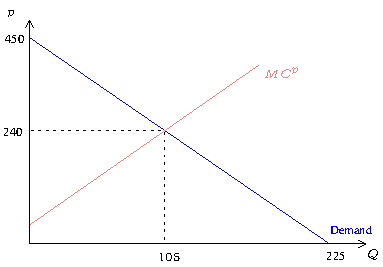
\includegraphics{pics/Ext1}
  \end{center}
\end{frame}

\begin{frame}
  \frametitle{Social costs}
  Marginal cost to society due to pollution:
\[
MC^g(Q) = Q.
\]

\uncover<2->{Social marginal cost:
\[
MC^s(Q) =  MC^p(Q) + MC^g(Q) \uncover<3->{ = 30 + 2Q + Q}\uncover<4->{ = 30+3Q.}
\]}
\uncover<5->{To find the social optimum, equate inverse demand and $MC^s$:

\[
30+3Q = 450 - 2Q
\]}
\uncover<6->{So $Q_s = 84$ and $p_s = 282.$}



\end{frame}

\begin{frame}
  \frametitle{Graphically} 
  \begin{center}
    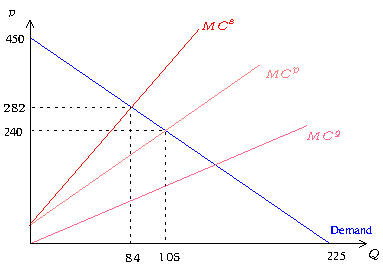
\includegraphics{pics/Ext2} 
  \end{center} 
\end{frame}

\begin{frame}
  \frametitle{Social welfare}
  Previously, we only needed to think about CS and PS.
\bigskip

\uncover<2->{Now we also consider the harm from pollution.}
\bigskip


\uncover<3->{\[W = CS + PS - \underset{\text{cost of pollution}}{C_g}\]}
\end{frame}


\begin{frame}
  \frametitle{Social welfare}
  \begin{center}
    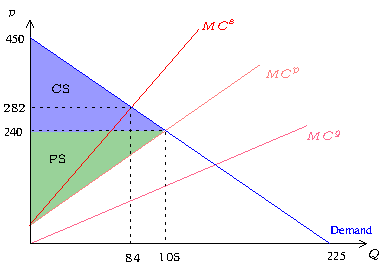
\includegraphics{pics/Ext3}
  \end{center}
If we ignore the social cost of pollution, welfare is CS+PS.
\end{frame}

\begin{frame}
  \frametitle{Social welfare}
  \begin{center}
    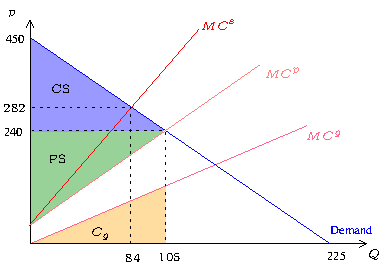
\includegraphics{pics/Ext4}
  \end{center}
The yellow area is the social cost of 105 units of pollution.
\end{frame}

\begin{frame}
  \frametitle{Social welfare}
  \begin{center}
    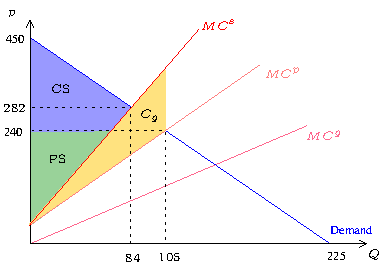
\includegraphics{pics/Ext5}
  \end{center}
Since $MC^s - MC^p = MC^g$, this is the same area.
\end{frame}


\begin{frame}
  \frametitle{Social welfare}
  \begin{center}
    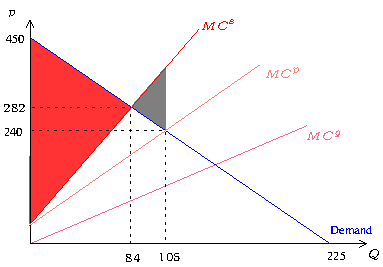
\includegraphics{pics/Ext6}
  \end{center}
Total welfare is the red area minus the grey area.
\end{frame}

\begin{frame}
  \frametitle{Social welfare}
  \begin{center}
    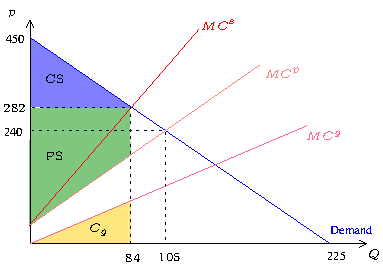
\includegraphics{pics/Ext7}
  \end{center}
Social optimum: total welfare is calculated as $CS+PS-C_g$.
\end{frame}

\begin{frame}
  \frametitle{Social welfare}
  \begin{center}
    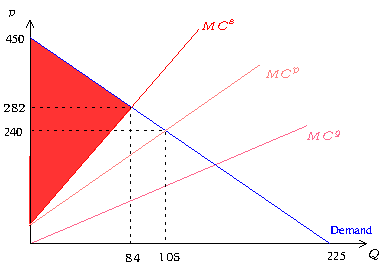
\includegraphics{pics/Ext8}
  \end{center}
So total welfare is the red area.
\end{frame}



\begin{frame}
  \frametitle{Social welfare}
  \begin{center}
    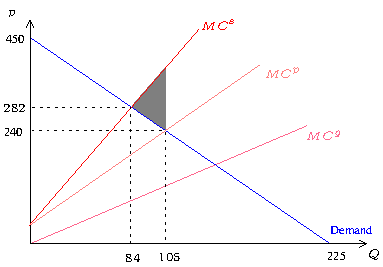
\includegraphics{pics/Ext9}
  \end{center}
Loss of welfare from competitive allocation is the grey area.
\end{frame}




\begin{frame}
  \frametitle{Cost-benefit analysis}
  Do negative externalities mean that we eliminate all pollution?

\bigskip

\uncover<2->{Cost of doing so: 
no paper.}

\bigskip
\uncover<3->{We must balance the costs and benefits of reducing pollution.}

\bigskip
\uncover<4->{$B(G)$ --- benefit to society from cutting pollution by $G$ from
$G_c$.}
\medskip

\uncover<5->{This is from reduced pollution.}
\bigskip

\uncover<6->{$C(G)$ --- cost to society from cutting pollution by $G$ from $G_c$.}

\uncover<7->{\medskip This is from reduced consumption.}





\end{frame}

\begin{frame}
  \frametitle{Cost-benefit analysis}
  To balance these, we pick the amount to cut that maximizes
\[
W(G) = B(G) - C(G).
\]
\uncover<2->{First order condition:
\[
\frac{dW}{dG} = \frac{dB}{dG} -\frac{dC}{dG} = 0.
\]}
\uncover<3->{In other words: 
\[
\frac{dB}{dG} =\frac{dC}{dG}.
\]}
\uncover<4->{The \emph{marginal} benefit equals the \emph{marginal} cost.}

\end{frame}

\begin{frame}
  \frametitle{Regulating externalities}
  Without regulation, we end up at the competitive outcome.

\bigskip
\uncover<2->{As we saw, there is too much of the good in a competitive equilibrium.}

\bigskip
\uncover<3->{Regulate to ensure the right amount.}
\bigskip

\uncover<4->{Two kinds of regulation:}
\begin{enumerate}
\item<5-> Standards: restrict the amount that the mills can pollute to
  84 units.
\item <6-> Taxes: charge a tax to make the private cost more like the
  social cost.
\end{enumerate}

\end{frame}

\begin{frame}
  \frametitle{Standards}
  Difficulties with standards:
  \begin{itemize}
    \item Need to know enough to calculate the optimal quantity. 
    \item Enforcement can be difficult.
  \end{itemize}
\end{frame}


\begin{frame}
  \frametitle{Taxes/fees}
  Cause paper mills to \emph{internalize} the externality.

\bigskip
\uncover<2->{If we know $MC^g$, set $\tau(Q) = MC^g(Q)$ --- pick specific tax to
exactly reflect the cost of the externality.}
\bigskip

\uncover<3->{Then, if mills are profit maximizing, in equilibrium
\[
MC^p(Q) + \tau(Q) = p.
\]}

\uncover<4->{This is particularly handy if firms can switch to technologies that
pollute less.}


\end{frame}

\begin{frame}
  \frametitle{Graphically}
  \begin{center}
    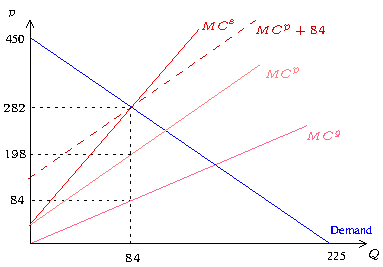
\includegraphics{pics/ExtTax}
  \end{center}
\end{frame}



\begin{frame}
  \frametitle{Market structure and externalities}
  Remember: monopolies usually produces less than the competitive
  quantity.

\bigskip
\uncover<2->{But this might still be more or less than the socially optimal
quantity.}


\bigskip
\uncover<3->{To maximize profit, monopoly paper mill equates $MC^p(Q)$ and 
\[MR(Q) = 450 - 4Q\]  }

\uncover<4->{$Q_m=70$ and $p_m=310$.}

\bigskip
\uncover<5->{Notice that $Q_m < Q_s$.}

\bigskip
\uncover<6->{But this calculation doesn't account for $MC^g(Q)$ so if
  social cost were much greater than private cost, the monopoly might produce too much.}

\end{frame}

\begin{frame}
  \frametitle{Monopoly ad externalities}
  \begin{center}
    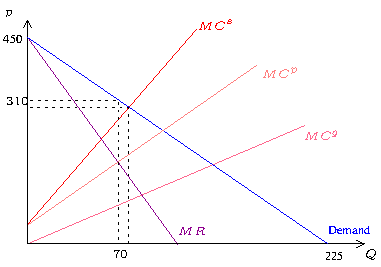
\includegraphics{pics/Monop1}
  \end{center}
In this case, the monopoly produces too little of good (despite the pollution).

\end{frame}
\begin{frame}
  \frametitle{Monopoly ad externalities}
  \begin{center}
    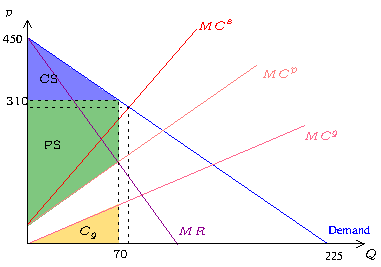
\includegraphics{pics/Monop2}
  \end{center}
To evaluate the impact of the monopoly, calculate social welfare.
\\
\
\end{frame}

\begin{frame}
  \frametitle{Monopoly ad externalities}
  \begin{center}
    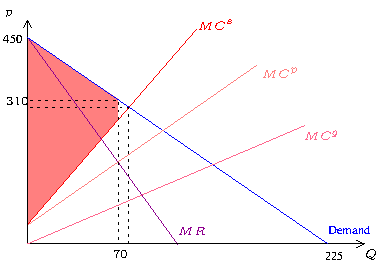
\includegraphics{pics/Monop3}
  \end{center}
Social welfare is the red area.
\\
\
\end{frame}
\begin{frame}
  \frametitle{Monopoly ad externalities}
  \begin{center}
    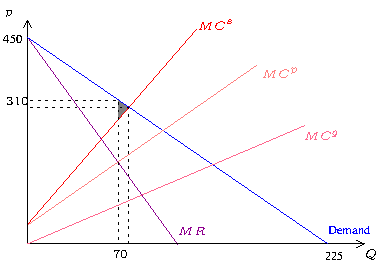
\includegraphics{pics/Monop4}
  \end{center}
Deadweight loss from monopoly is the grey area.
\\
\
\end{frame}

\begin{frame}
  \frametitle{Monopoly ad externalities}
  \begin{center}
    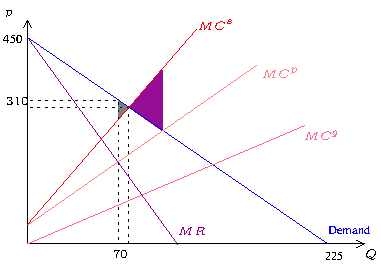
\includegraphics{pics/Monop5}
  \end{center}
DWL from monopoly (grey) is less than 
competition (purple). \uncover<2->{Relationship can go the other way
  for other $MC$s and $D$.}

\end{frame}


\begin{frame}
  \frametitle{Tax, monopoly, and externalities}

If the tax is chosen so that  $\tau(Q) = MC^g(Q)$, the monopoly can
affect the tax rate.

\bigskip
\uncover<2->{So $MC(Q) = MC^p(Q) + \tau(Q)$.}

\bigskip
\uncover<3->{The monopoly completely internalizes the cost of pollution.}

\bigskip
\uncover<4->{If there was underprovision without a tax the situation will be
worsened by the tax.}

\bigskip
\uncover<5->{But if there was overprovision without tax, the tax \emph{may} help.}
\end{frame}



\begin{frame}
  \frametitle{Tax, monopoly, and externalities}
  \begin{center}
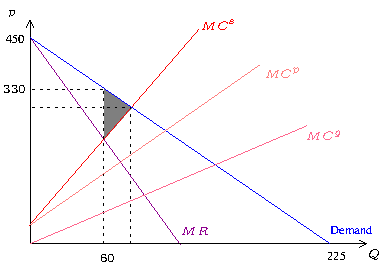
\includegraphics{pics/Monop6}
  \end{center}
DWL is higher with tax than without. 
\end{frame}

\begin{frame}
  \frametitle{Allocating property rights}
  The lack of property rights is a problem.

\bigskip
\uncover<2->{If you had the right to clean air, you can sell that to a
polluter: the polluter then internalizes the harm of his pollution
because he would have to pay you.}

\bigskip
\uncover<3->{the \emph{Coase} Theorem: if property rights are specified, the
polluter and its victim can bargain and end up with the optimal level
of pollution.}

\bigskip
\uncover<4->{Not a practical solution, but highlights the problem of not having
property rights defined.}


\end{frame}


\begin{frame}
  \frametitle{Coasian bargaining}
  Mechanic and tea house next to one another.\bigskip

\uncover<2->{Fixing cars is noisy and hurts the tea house's business.}
\bigskip
\begin{center}
  
\uncover<3->{\begin{tabular}{|c|ccc|}
\hline  Cars per hour & $\pi_{mech}$ & $\pi_{tea}$ & total\\
\hline 0 & 0 & 400 & 400\\
\hline 1 & 300 & 200 & 500\\
\hline 2 & 400 & 0 & 400\\
\hline
\end{tabular}}
\end{center}

\uncover<4->{Social optimum: 1 car per hour and total profit of 500.}

\end{frame}

\begin{frame}
  \frametitle{Coasian bargaining}
\begin{center}
  
\begin{tabular}{|c|ccc|}
\hline  Cars per hour & $\pi_{mech}$ & $\pi_{tea}$ & total\\
\hline 0 & 0 & 400 & 400\\
\hline 1 & 300 & 200 & 500\\
\hline {\color{red} 2} &{\color{red} 400} & {\color{red} 0} & {\color{red} 400}\\
\hline
\end{tabular}
\end{center}
If no property rights: mechanic maximizes profits by choosing to work
on 2 cars per hour.
\end{frame}

\begin{frame}
\frametitle{Coasian bargaining}
\begin{center}
\begin{tabular}{|c|ccc|}
\hline  Cars per hour & $\pi_{mech}$ & $\pi_{tea}$ & total\\
\hline 0 & 0 & 400 & 400\\
\hline {\color{red} 1} &{\color{red} 300} & {\color{red} 200} & {\color{red} 500}\\
\hline 2 & 400&0 & 400\\
\hline
\end{tabular}
\end{center}
Right to quiet:
tea house  maximizes profit by selling the
right to one car per hour for 200. The mechanic makes 300 minus the
200 paid for the right to work on a car. The tea shop makes 200 plus
the 200 it gets from the mechanic.


\end{frame}


\begin{frame}
\frametitle{Coasian bargaining}
\begin{center}
\begin{tabular}{|c|ccc|}
\hline  Cars per hour & $\pi_{mech}$ & $\pi_{tea}$ & total\\
\hline 0 & 0 & 400 & 400\\
\hline {\color{red} 1} &{\color{red} 300} & {\color{red} 200} & {\color{red} 500}\\
\hline 2 & 400&0 & 400\\
\hline
\end{tabular}
\end{center}
Right to be noisy: mechanic sells its right to work on one car and makes
300. The loss of 100 is made up for by the price it charges the tea shop
between 100 and 200.


\end{frame}
\begin{frame}
  \frametitle{Coasian bargaining}
Summary:  \begin{enumerate}
  \item<2-> No property rights: inefficient.
  \item<3-> Clearly property rights: efficient no matter the
    allocation of the rights.
  \item<4-> Allocation of property rights matters for how well off
    each person is.
  \end{enumerate}
\bigskip

\uncover<5->{Caveat: This kind of bargaining only works in very special
  circumstances where there is no asymmetric information, no
  transaction cost, and so on.}
\end{frame}


\begin{frame}
  \frametitle{Rivalry and exclusion}
\emph{Rivalry:} Only one person can consume a good.

\bigskip
\uncover<2->{An apple is rivalrous. Clean air, national defense, etc. are not.}
\bigskip


\uncover<3->{  \emph{Exclusion:} One can be prevented from consuming a good.}

\bigskip
\uncover<4->{You can lock the apple in a safe to prevent other people
  from using it. You can't prevent someone from breathing clean air.}

\bigskip
\uncover<5->{\begin{center}
  \begin{tabular}{c|c|c|}
    & Exclusion & No exclusion\\
\hline
Rivalry &  Private goods & Common goods\\
\hline 
No Rivalry & Club goods & Public goods\\
\hline   \end{tabular}
\end{center}}
\uncover<6->{Markets for all but private goods fail.}
\end{frame}

\begin{frame}
  \frametitle{Common goods}
  (Open access) common goods can be used by anyone.

\bigskip
\uncover<2->{Use by one makes the good unavailable for others.}

\bigskip

\uncover<3->{Examples: Fisheries,  public roads, ``commons''.}

\bigskip

\uncover<4->{Since there are no property rights common goods are over-used.}

\bigskip
\uncover<5->{This is the \emph{tragedy of the commons}.}
\end{frame}

\begin{frame}
  \frametitle{Club goods}
Examples:  Cable TV, software.

\bigskip
\uncover<2->{Zero marginal cost to provide the good to additional customers.}
\bigskip

\uncover<3->{At any price (above zero) there is deadweight loss: market failure.}
\bigskip

\uncover<4->{Cannot regulate to require price to be zero.}
\end{frame}


\begin{frame}
  \frametitle{Public goods}
  Everyone consumes public goods.

\bigskip
\uncover<2->{Example: hiring  a security guard.}

\bigskip
\uncover<3->{Two stores next too one another $1$ and $2$.}

\bigskip
\uncover<4->{Benefit from a guard: 8 to each.}
\bigskip

\uncover<5->{Cost of a guard: 10 for whoever hires.}

\bigskip
\uncover<6->{So if $1$ hires and $2$ doesn't:

 $1$ gets $8-10=-2$ 

$2$ gets $8-0=8$.}
\end{frame}


\begin{frame}
  \frametitle{Hiring game}
\begin{center}  \begin{tabular}{c|c|c|}
    & $2$ hires & $2$ doesn't hire\\
\hline $1$ hires & $-2$, $-2$ & $-2$, 8 \\
\hline $1$ doesn't hire  & 8, $-2$ & 0, 0\\
\hline 
  \end{tabular}
\end{center}
\uncover<2->{Nash equilibrium:  Neither hires.}
\bigskip


\uncover<3->{\emph{Free riding}: I'll just let the other one do it.}

\bigskip
\uncover<4->{If you have a roommate, this is what probably happens when it comes to
cleaning up.}
\end{frame}


\begin{frame}
  \frametitle{What if they split the cost?}
  Rather than both hiring, they pay 5 a piece. So if both agree to
  hire, each gets $8-5 = 3$.
\uncover<2->{\begin{center}  \begin{tabular}{c|c|c|}
    & $2$ hires & $2$ doesn't hire\\
\hline $1$ hires & $3$, $3$ & $-2$, 8 \\
\hline $1$ doesn't hire  & 8, $-2$ & 0, 0\\
\hline 
  \end{tabular}
\end{center}}
\bigskip

\uncover<3->{The Nash equilibrium is still for neither to hire.}

\end{frame}

\begin{frame}
  \frametitle{A more general example}
The number of guards can be varied.

\bigskip
\uncover<2->{Store 1's inverse demand, $D^1(q)$, is the value of the $q^{th}$
guards to it}.

\bigskip
\uncover<3->{Total value of $q$ guards: $D^1(q) + D^2(q)$ --- vertical sum.}

\end{frame}



\begin{frame}
  \frametitle{Free riding}
  \begin{center}
    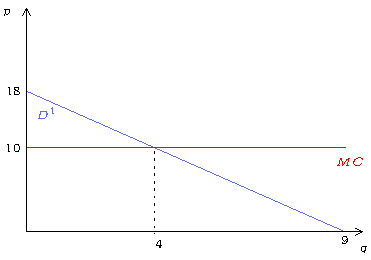
\includegraphics{pics/FreeRiding1}
  \end{center}
If 1 makes its decision alone, with no guards provided by 2, it
decides on 4 guards.
\end{frame}

\begin{frame}
  \frametitle{Free riding}
  \begin{center}
    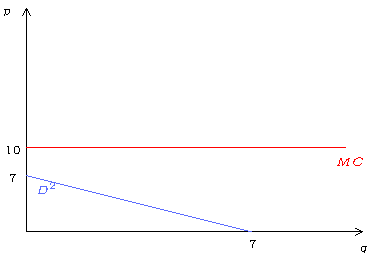
\includegraphics{pics/FreeRiding2}
  \end{center}
If 2 makes its decision alone, with no guards provided by 1, it
decides on no guards.
\end{frame}

\begin{frame}
  \frametitle{Social optimum}
  \begin{center}
    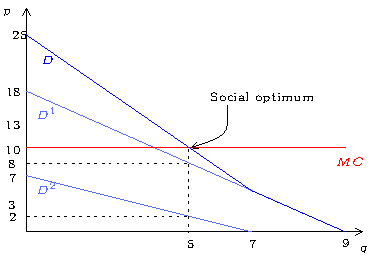
\includegraphics{pics/FreeRiding3}
  \end{center}
The social optimum is to hire 5 guards and split the cost between 1
and 2. 
\end{frame}

\begin{frame}
  \frametitle{Equilibrium}
  \begin{center}
    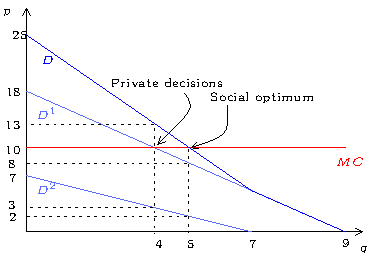
\includegraphics{pics/FreeRiding}
  \end{center}
If they are choosing independently, the equilibrium is for 1 to hire 4
guards and 2 to hire none. 
\end{frame}





\begin{frame}
  \frametitle{Efficient level of a public good}
  $U_1(G, P_1)$ --- utility of store 1 with $G$ guards while paying 
  $P_1$.\bigskip

\uncover<2->{  $U_2(G, P_2)$ --- utility of store 2 with $G$ guards while paying
  $P_2$.\bigskip}

\uncover<3->{$G = G_1+G_2$ --- the total amount of public good  provided.}

\bigskip

\uncover<4->{Pareto-efficiency: Each provides $G_i$ so that  increasing one's
utility decreases the other's.}

\end{frame}
\begin{frame}
  \frametitle{Pareto-efficiency}
We can prove (won't do it here) that an allocation is
Pareto-efficient when 
\[
MRS_1 + MRS_2 = \text{price of a guard.}
\]
\uncover<2->{This is the \emph{Samuelson condition.} Compare with efficiency
condition for private goods ($MRS_1 = MRS_2$).}

\bigskip
\uncover<3->{The difference comes from the absence of rivalry: you have to add up
utilities. It's not one or the other.}

\bigskip

\uncover<4->{Free riding leads to the phenomenon where the provision of the public
good is too little if we treat it like a private good.}


\end{frame}


\begin{frame}
  \frametitle{What to do about free riding}
  This is a market failure where government intervention and other
  social institutions can help:
  \begin{enumerate}
  \item<2-> Social pressure: in a repeated game, we saw that
    non-contribution can be punished over time.
  \item<3-> Mergers: free riding can be avoided among firms if they
    are seek to maximize total profits rather than individual profits.
  \item<4-> Contracts: we can stop short of merging if the firms can
    agree to sign contracts to guarantee that they cooperate.
  \item<5-> Coercion: the government can impose the socially efficient
    levels via taxes.
  \end{enumerate}
\end{frame}



\end{document}







